%Put this in order they appear in beamline?
\section{Beamline Components}

The Hall A Beamline has several measurement devices that allow the experimenter to fully understand the beam that is being delivered to the hall. For positioning, there are the Beam Position Monitors and the Harp. For beamspot sizing, there is the raster. For current and charge measurements, there are the Beam Current Monitors.

\subsection{Beam Position Monitors}

The Beam Position Monitors (BPMs) are a pair of measurement devices that consist of four sensing wires. By calibrating the signal received from each wire, the experimenter can reconstruct the position of the beam as it passed the BPM. Using both BPMs in conjunction allows the experimenter to determine the beam trajectory and where the electrons are incident on the target.

The BPMs are calibrated using a Harp fork. The Harp consists of three wires that are introduced sequentially into the path of the beam using a stepper motor. When the beam is incident on a wire, a charge is induced. By determining when each wire is struck by the beam, the experimenter can very accurately determine the position of the beam. This is an invasive measurement.

\subsection{Raster}
\begin{figure}
	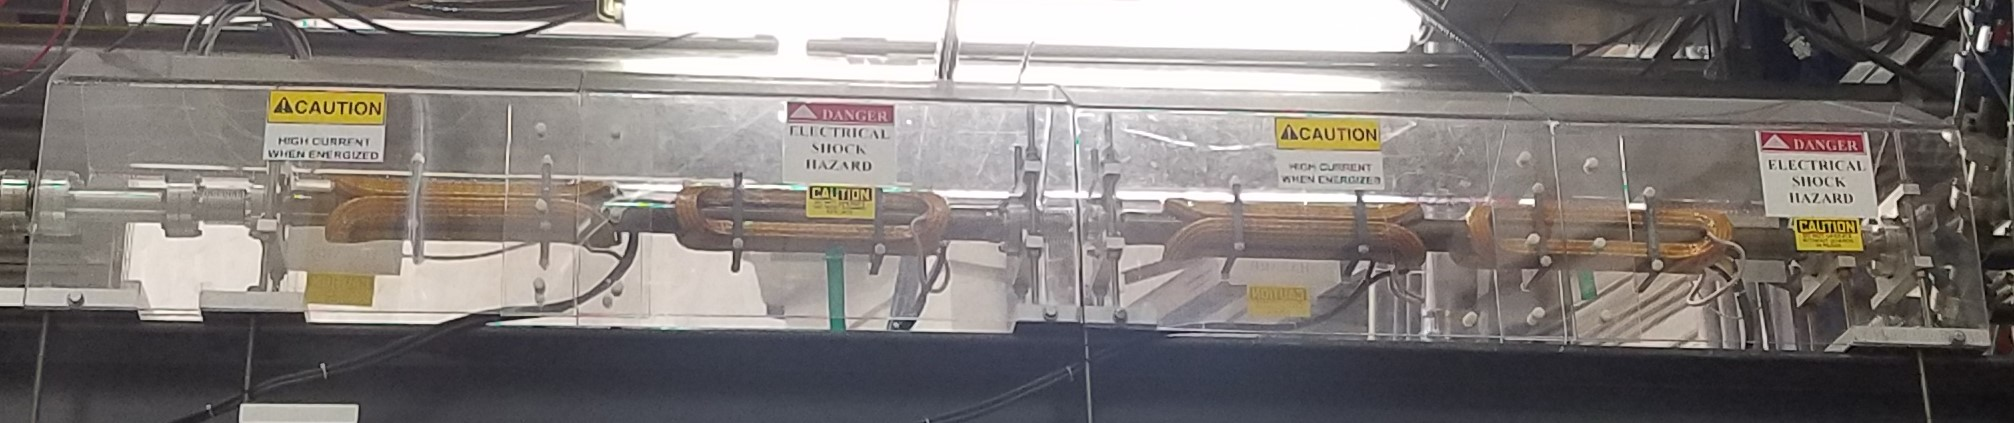
\includegraphics[width=\linewidth]{./chap2-exp/fig/raster_pic.jpg}
	\caption{The Hall A raster consists of four dipole magnets on the beamline}
	\label{fig:rasterpic}
\end{figure}

When the beam enters Hall A it has very little spread, all of the electrons will strike the target in one small location. For solid targets, this poses no problem. However, for gas targets with thin cell walls localized heating can run the risk of a cell rupture. The raster exists in the beamline to mitigate this risk. The raster is a set of four dipole magnets: two for steering horizontally (x) and two for steering vertically (y).

The magnet pairs that work in the same direction are synced, which ensures that they maximize the beam spread and do not work against each other. Each raster magnet is powered by a triangle wave of different frequencies to minimize harmonics. The horizontal rasters are set to 24.5 kHz and the vertical rasters are set to 25 kHz \cite{rast_current}. The triangle wave ensures that equal time is spent at all points in the rastered area. Figure \ref{fig:exrast} shows a typical raster spectrum as recorded by the High Resolution Spectrometer (HRS).

\begin{figure}
	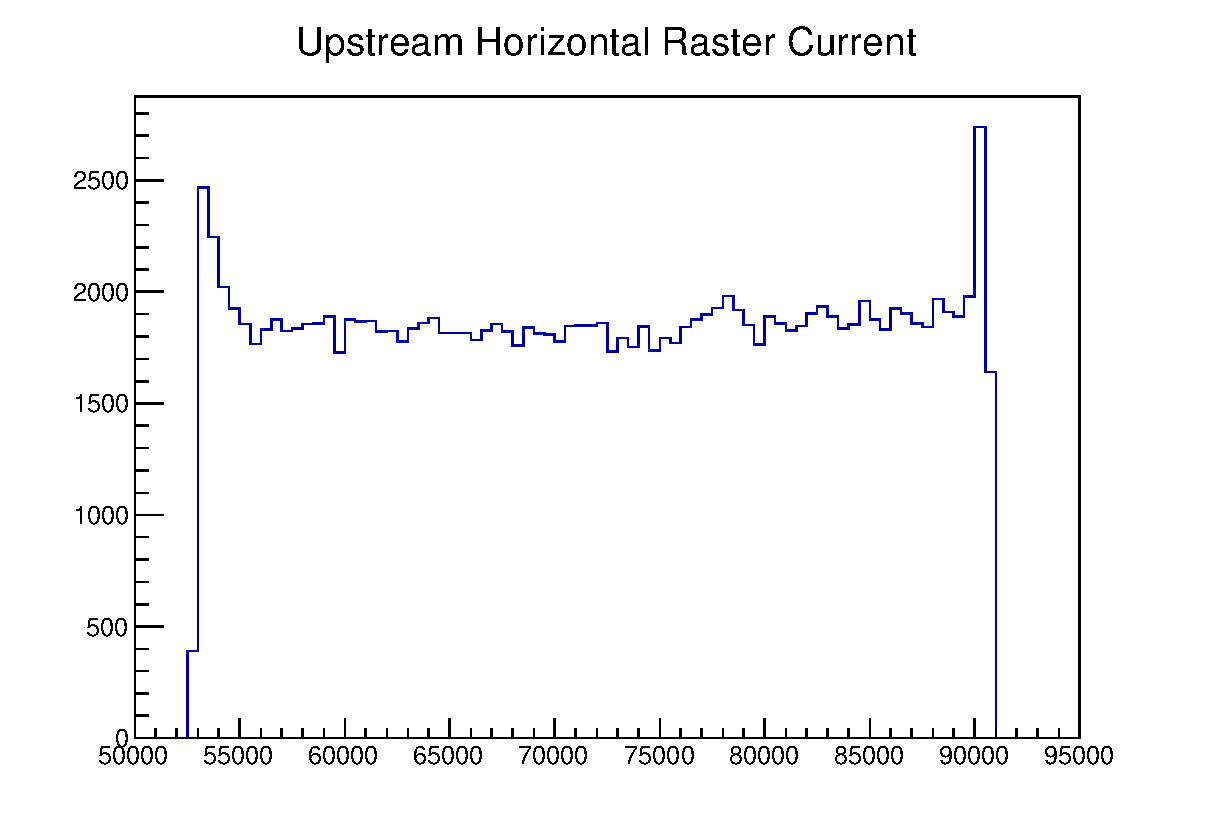
\includegraphics[width=\textwidth]{./chap2-exp/fig/ex_rast.eps}
	\caption{An example of a raster current spectrum. The range and size will change with ADCs used, beam energy, and raster size. The shape should always stay the same. The ``bedposts'' on the edges are due to rounding of the triangular waveform by a low-pass filter.}
	\label{fig:exrast}
\end{figure}

\begin{figure}
	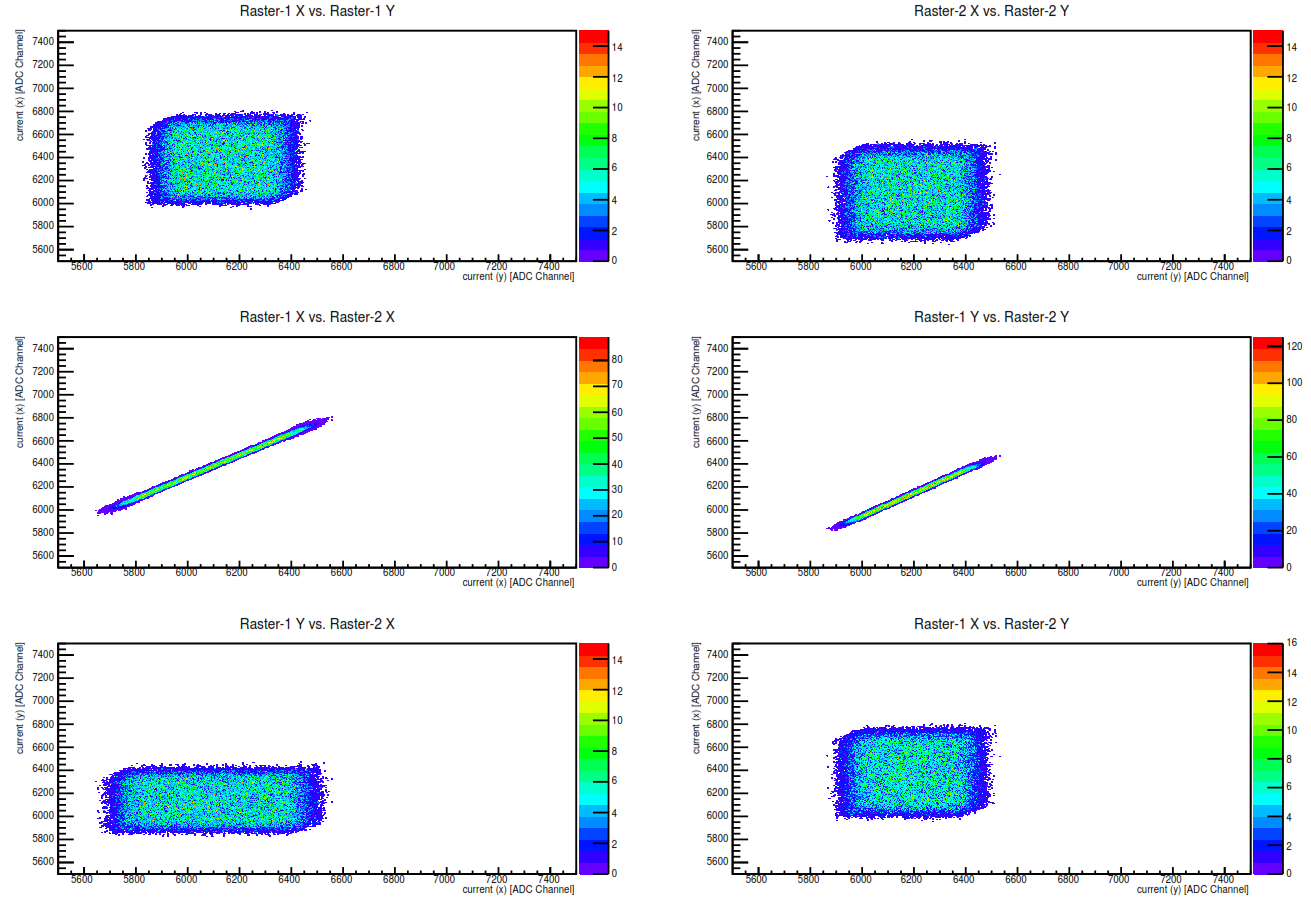
\includegraphics[width=\linewidth]{./chap2-exp/fig/raster_sync.png}
	\caption{The X and Y raster pairs are each synced to produce the maximum kick. The X and Y directions are uncorrelated so that the beam travels uniformly over the target.}
	\label{fig:raster}
\end{figure}

\subsection{Beam Current Monitor}

The Hall A Beam Current Monitor (BCM) is comprised of an Unser monitor and two RF cavities. The Unser provides an absolute reference for the RF cavities. The calibration of the Unser drifts quite quickly, so it is used to calibrate the RF cavities but cannot be used for long-term monitoring.

Each RF cavity is tuned to the frequency of the beam (1.497 GHz). The resonance then produces a voltage proportional to the beam current. The signals are then split to be either sampled or integrated. The sampled signal outputs the RMS of the voltage over a 1 second period. This is equivalent to the average beam current for that second. The signal that is integrated is first sent to an RMS-to-DC converter which is then fed to a Voltage-to-Frequency converter. This signal is then sent to a scalar that accumulates over a run. The final scalar value is proportional to the total accumulated charge in the run.